% !TeX root = main.tex
% !TeX spellcheck = fa_IR
%\chapter{مواد و روش‌ها} % برای پژوهش‌های تجربی یا
%\chapter{الگوریتم‌ها  و روش‌ها} % الگوریتم‌ها و روش‌ها در پژوهش‌های عددی
\chapter{روش‌ها}
اگر پروژه شما تجربی باشد، در این فصل به معرفی کلی مواد و روش‌های استفاده شده پرداخته می‌شود. این بخش باید به گونه‌ای نوشته شود که خواننده بتواند روند کلی پژوهش را درک کند. در ادامه، احتمالاً بخشی به مواد اختصاص می‌یابد که در آن فهرستی از مواد اولیه مورد استفاده (شامل مواد شیمیایی، نمونه‌ها، غیره) و ویژگی‌های آنها ذکر می‌شود. سپس ابزارهای مورد نیاز فهرست می‌شوند و بخش بعدی به روش آماده‌سازی مواد، روش‌های آزمایش و تحلیلی نتایج  اختصاص می‌یابد. نهایتا بخشی نیز به جمع‌بندی مطالب این فصل اختصاص می‌یابد.

اگر پروژه شما محاسبات عددی یا شبیه‌سازی باشد، ترتیب مطالب این فصل تفاوت چندانی ندارد. فقط به‌جای مواد و ابزارها از روش‌ها و الگوریتم‌ها صحبت خواهید کرد و ویژگی‌ها و تفاوت‌های آنها را بیان خواهید کرد. باز هم باید مطالبی در مورد تحلیل نتایج و داده‌ها داشته باشید و سرآخر جمع‌بندی خواهید داشت.

در ادامه این فصل به بیان روش نگارش پایان‌نامه یا رساله با استفاده از سیستم حروف‌چینی 
\xelatex\LTRfootnote{\XeLaTeX} 
و زیرمجموعهٔ آن بستهٔ 
\xepersian\LTRfootnote{\XePersian} 
می‌پردازیم. توضیحات و راهنمایی‌ها با نمونه و مثال ارائه می‌شوند تا کار نگارش اصطلاحات علمی، عبارت‌ها و روابط ریاضی، شکل‌ها و جداول را برایتان ساده کنند. 

مهمترین کاری که باید بتوانید انجام دهید، ارجاع درست به پژوهش‌های پیشین است. این مراجع ممکن است مقاله 
\cite{myers2013improving}، 
کتاب 
\cite{willey2008prescott}، 
پایان‌نامه کارشناسی ارشد 
\cite{Iri}، 
رسالهٔ دکتری 
\cite{Mostafavi}، 
یا صفحات تارنما%
\LTRfootnote{webpages} 
باشند 
\cite{thesis}. 
شیوه ارجاع در متن به همهٔ آنها یکسان است، اما قالب هریک تفاوت‌های کوچکی دارد. اینجا از هریک مثالی آورده‌ایم تا شما بتوانید با مراجعه به فایل 
\lr{`MyReferences.bib'} 
تفاوت‌ها را ببینید. این روزها دانشجویان فراوان به دانشنامه‌های آنلاین نظیر دانشنامهٔ آزاد ویکی‌پدیا ارجاع می‌دهند. در این موارد فراموش نکنید که از لینک دائمی به صفحه استفاده کنید تا تغییرات زمانی صفحات آنلاین مرجع شما را مخدوش نکند.

برای نگارش 
\thesis 
ممکن است مفاهیم و کمیت‌هایی را از منابع دیگر یادبگیرید و به‌کارگیرید. ممکن است در مستندات علمی نمادها و نشانه‌های متفاوتی برای این کمیت‌ها متداول باشد و منبعی که از آن استفاده می‌کنید، یکی از آنها را به‌کار گرفته باشد. شما اجازه ندارید به دو کمیت یا مفهوم متفاوت یک نماد اختصاص دهید، بنابراین لازم است متناسب با کمیت‌ها و مفاهیم به‌کار رفته در نوشتارتان و میزان تکرار هر مفهوم الگوی سازگاری از نمادها را به کمیت‌ها اختصاص دهید که یکتا و با مسما باشد. فهرست نمادها می‌تواند در انتخاب نمادهای غیر تکراری به شما کمک کند. برای مثال $w$ برای نشان دادن پهنا، وزن و کار استفاده می‌شود. از هر سه کمیت نیاز باشد، می‌توان پهنا را با $w$ نشان داد، وزن را با $W$ و کار را با
$\mathcal{W}$. 
به این ترتیب با حفظ سازگاری همه کمیت‌ها قابل تشخیص خواهند بود. این کمیت‌ها را می‌توان به فهرست نمادها نیز اضافه کرد.
\addsymbolslist{$w$}{پهنا}
\addsymbolslist{$W$}{وزن}
\addsymbolslist{$\mathcal{W}$}{کار}

به مرور که در متن با نمادهای جدید روبرو می‌شوید، آنها به فهرست اضافه کنید. به این ترتیب می‌توانید با مرور فهرست نمادهای بعدی را راحت‌تر انتخاب کنید. 
اگر تعداد نمادها در 
\thesis 
شما خیلی زیاد است و از طرفی تعریف آنها طولانی نیست، می‌توانید با دستور 
$\backslash\texttt{twocolumnsymbolslist}$ 
فهرست نمادها را دو ستونه کنید، زیرا فضای خالی سمت چپ صفحات فهرست زیبا به نظر نمی‌رسد.

\normalfootnotes
معمولاً از زیرنویس برای معرفی معادل انگلیسی اصطلاحات و واژه‌های جدید و همچنین نام پژوهشگران استفاده می‌کنیم. به همین دلیل بیشتر زیرنویس‌ها تنها به اندازهٔ یک واژه طول دارند. اگر تعداد زیرنویس‌ها در یک صفحه زیاد باشد، چند سطر خالی در پایین صفحه ظاهر می‌شود که زیبا نیست. در پاورقی‌ها این الگو معادل انگلیسی واژه‌ها در دو ستون مرتب شده است تا فضای خالی در پایین صفحات ایجاد نشود. اما گاهاً ناچاریم یک توضیح یا تعریف نا مرتبط با سیر منطقی بحث را برای خواننده در پاورقی بیاوریم. چنین توضیحاتی در نیم خط نمی‌گنجند%
\footnote{
وقتی می‌خواهیم یک زیرنویس طولانی چند خطی داشته باشیم. بهتر است، موقتاً زیرنویس‌ها را یک ستونه کنیم و بعد دوباره آنها را به حالت دو ستونه برگردانیم. در اینجا عمداً این توضیح را در پاورقی آوردیم، تا به‌عنوان یک نمونه قابل استفاده باشد.}.
\twocolumnfootnotes

لزومی ندارد تمام این فصل را کامل مطالعه کنید. ابتدا روش‌های ساده را یاد بگیرید و کار نگارش 
\thesis  
را شروع کنید. هر زمان با مشکلی مواجه شدید، می‌توانید به محتوی این فصل نگاهی بیاندازید و از مثال‌های آن استفاده کنید.


\section{قواعدی ساده در نگارش متن}
در گذشته زمانی که حروف‌چینی و چاپ آغاز شد برای کاهش هزینه‌ها افراد ناوارد کار حروف‌چینی را انجام می‌دادند. همین مسأله سبب شد، همزه و 'ی` نکره که بعد از 'ـه` آخر می‌آمد با حروف یکسان حروف‌چینی شود. بعدها برای آگاهی عموم فارسی‌زبان‌ها پیشنهاد شد که 'ی` نکره به صورت کامل نوشته شود، مثلاً بنویسیم 'مسأله‌ی` یا 'معادله‌ی`. بعد از مدتی متوجه شدیم در گذشته‌های دور وقتی هنرمندان خطاط می‌خواستند 'ی` نکره را بنویسند، آن را خیلی کوچک بالای 'ـه` آخر می‌گذاشتند.  به همین سبب، امروزه نیز توصیه می‌شود، اگر محیط نگارش اجازه می‌دهد، به رویه گذشته عمل کنیم. خوشبختانه نسخه‌های اخیر بستهٔ حروف‌چینی 'بای‌دی`%
\LTRfootnote{\textsf{bidi} (bidirectional typesetting)}
که 
\xepersian 
از آن بهره می‌برد، به شرط نصب قلم‌های استاندارد فارسی، این قابلیت را دارد. بنابراین بهتر است به‌جای مسأله‌ی بنویسیم "مسألهٔ``. به تفاوت علامت همزه (ء) و 'ی` کوچک در این واژه دقت کنید.

در نگارش متن فارسی، رایج است که کلمات مرکب، پیشوندها و پسوندها با نیم‌فاصله نوشته شوند. نیم‌فاصله یا به عبارت درست‌تر فاصله مجازی%
\LTRfootnote{Zero-width non-joiner (ZWNJ)} 
در جانمایی‌های%
\LTRfootnote{keyboard layouts} 
مختلف صفحه‌کلید با ترکیب متفاوتی از کلیدها تایپ می‌شود، مثلاً:
\lr{Shift+Space}، \lr{Ctrl+Shift+2}، \lr{Shift+b}، یا \lr{Alt+0157}. 
در آخرین مورد، اعداد را باید با صفحه‌کلید عددی%
\LTRfootnote{numpad} 
تایپ کنید. اگر هیچ یک از این ترکیبات برای شما کار نمی‌کند، خودتان می‌توانید برای آن یک میانبر تعریف کنید. 

در نگارش برخی کلمات مرکب مثل اسامی خاص، بهتر است از خط تیره (-) به‌جای نیم‌فاصله استفاده شود. مثلاً بهتر است بنویسیم مدل کاردر\dash پاریزی\dash ژانگ%
\LTRfootnote{Kardar-Parisi-Zhang}. 
این علامت را با خط تیره طویل (--) که برای نشان دادن یک بازه استفاده می‌شود اشتباه نگیرید، مثلاً سال‌های ۱۳۶۸--۱۳۵۸. خط تیره بسیار طولانی (---) هم برای مشخص کردن جملات معترضه استفاده می‌شود. مثلاً، دقت در انجام پژوهش ---گرچه زحمت زیادی دارد--- به نتایج افتخار آمیز منجر می‌شود. در فارسی خط کرسی نیز هست که برای کشــــــیده نوشتن کلمات استفاده می‌شود.

گاهی احتیاج خواهید داشت که از گیومه برای نقل قول یا برجسته کردن یک واژه استفاده کنید. انتخاب الگوی "انگلیسی`` یا «فرانسوی» به سلیقه شما بستگی دارد، اما بهتر است از الگوی یکسانی برای تمام متن استفاده کنید. گیومه را می‌توان 'یگانه` یا "دوگانه`` گذاشت. به جهت چرخش و تفاوت نماد گیومه در دو طرف واژه توجه کنید. این ظرافت‌ها اگرچه در مفهوم مطلبی که می‌نویسید بی‌اثر است، اما توجه و وسواس شما خواننده را از دقت و مهارت شما در انجام پژوهشی که به آن پرداخته‌اید، مطمئن می‌سازد. یک راه ساده‌تر برای برجسته کردن بخشی از متن 
\emph{ایرانیک} 
نوشتن آن است.

اصلی‌ترین دلیل استفاده از گیومه نقل قول است. ما معمولاً مفاهیم و روابط را با زبان خودمان بیان می‌کنیم و تنها برای جزئیات و سندیت موضوع به دیگران ارجاع می‌دهیم. اما ممکن است برای نشان دادن اهمیت یک موضوع، بیان فرد دیگری را عیناً به عاریت بگیریم. مثلاً، در ابتدای مقدمه یک
\thesis 
در زمینه تلاطم برای رساندن اهمیت و پیچیدگی مسأله، چند جمله‌ای منتسب به وِرنر هایزنبرگ%
\LTRfootnote{Werner Heisenberg} 
را نقل کنیم تا خواننده را به هیجان آوریم. این چند جمله می‌تواند به زبان انگلیسی باشد:
\lr{\begin{quote}
``When I meet God, I am going to ask him two questions: Why relativity? And why turbulence? I really believe he will have an answer for the first." \cite{Wiscombe2005}
\end{quote}}
یا به فارسی ترجمه شده باشد:
\begin{quote}
«وقتی خداوند را ملاقات کنم، دو سوال از او خواهم پرسید: چرا نسبیت؟ و چرا تلاطم؟ واقعاً باور دارم که او برای اولین سوال پاسخ خواهد داشت.» 
\cite{Wiscombe2005}
\end{quote}
این‌که کدام را ترجیح دهیم به متن نقل قول و خواننده هدف بستگی دارد و اندکی سلیقه‌ای است. حتی ممکن است، یکی را در متن اصلی و دیگری را در پاورقی بیاوریم. مهم این است که متن نقل قول در گیومه و در محیط 
\lr{``quote"} 
آورده شود تا پهنای آن نسبت به متن اصلی کاهش یابد و به وضوح از متن 
\thesis 
متفاوت و قابل تشخیص و تفکیک باشد.


\section{نگارش روابط ریاضی}
در این الگو برای نگارش اعداد از قلم 'یاس` استفاده می‌کنیم، زیرا صفر آن توخالی است. برای مثال عدد 
$100$
را ببینید. برای مقادیر عددی دارای واحد نظیر،
$30.2\unit{mm}$ 
یا
$T_\mathrm{r} = 24\unit{\degC}$
می‌توانید از دستور ساده 
$\backslash\mathrm{unit}\{\mbox{\small\rl{واحد}}\}$ 
استفاده کنید. دقت کنید که در محیط فرمول پارامترها 
\textit{ایتالیک} 
نوشته می‌شوند. اما هرچیز مخفف یک کلمه باشد، بایستی به‌صورت طبیعی رومی%
\LTRfootnote{roman} 
نوشته شود. مثلاً واحدها (میلی‌متر، سانتیگراد و جز این‌ها)، نام توابع ریاضی (سینوس، کسینوس، و غیره)، یا نام عناصر شیمیایی را 
\textit{ایتالیک}  
نمی‌نویسیم،
\begin{equation*}
\mathrm{H}_2 + \tfrac{1}{2}\mathrm{O}_2 \longrightarrow \mathrm{H_2O}.
\end{equation*}

برای تبدیل فوریه تابع 
$f(x)$، 
می‌توان نوشت
$\mathcal{F}[f(x)]$.
این نمونه‌ای از یک رابطهٔ ریاضی داخل متن است. سعی کنید در متن، عبارات ریاضی را تا حد ممکن بدون توان و خط کسری بنویسید تا فاصله خطوط متن یکنواخت بماند و قلم عبارت‌های ریاضی نیز خیلی ظریف نشود. مثلاً به‌جای 
$L^{-1}$ یا $\frac{1}{L}$ 
در متن بنویسید، 
$1/L$.

ممکن است بخواهیم یک رابطه را در یک خط جدا بنویسیم. مثلاً،
\begin{equation}\label{eq1:1}
f(r) = \int_0^r \int_0^\pi r\sin\theta \d r \d\theta,
\end{equation}
یا برخلاف رابطهٔ~
\eqref{eq1:1} 
بخواهیم تعریف ماتریس پاولی را بدون شماره بیاوریم،
\begin{equation*}
\sigma_1 = \left(\begin{array}{ll}
0 & 1\\
1 & 0
\end{array}\right).
\end{equation*}
علامت '$*$` در کنار نام محیط 
\lr{`equation'} 
سبب شده، رابطه شماره نخورد. می‌توان یک رابطهٔ گسسته را هم نوشت، مثلاً 
$\sum_{i=1}^{n}x_i$.

در ادامه به عنوان نمونه دیگر، یک رابطهٔ سه‌خطی می‌آوریم،
\begin{eqnarray}\label{eq1:2}
h(x) &=& \int x^2\left(1+x^2\right) \d x\nonumber\\
&=& \tfrac{1}{3} x^3 + \tfrac{1}{5} x^5 + C,\\
q(x) &=& \frac{1}{1+\exp(-\beta x)}.\label{eq1:3}
\end{eqnarray}
دستور  
$\backslash\texttt{nonumber}$ 
سبب شد، خط اول رابطهٔ~%
\eqref{eq1:2} 
شماره نخورد. به ردیف شدن علامت‌های تساوی در سه‌خط رابطه توجه کنید. این نتیجه درج علامت‌های تساوی میان دو علامت 
'$\&$` 
است. همچنین ببینید که چگونه اندازه پرانتزها در خط اول با محتوی هماهنگ گشته است. این نتیجهٔ استفاده از پیشوندهای
$\backslash\texttt{left}$ و $\backslash\texttt{right}$ 
به‌ترتیب قبل از پرانتز باز و بسته است.

حالا یک رابطهٔ سه‌خطی برداری می‌آوریم،
\begin{subequations}\label{eq1:4}
\begin{eqnarray}
\mathbf{b}_1 &=& \frac{\mathbf{a}_2 \times \mathbf{a}_3}{\mathbf{a}_1.(\mathbf{a}_2 \times \mathbf{a}_3)},\label{eq1:4a}\\
\mathbf{b}_2 &=& \frac{\mathbf{a}_3 \times \mathbf{a}_1}{\mathbf{a}_1.(\mathbf{a}_2 \times \mathbf{a}_3)},\label{eq1:4b}\\
\mathbf{b}_3 &=& \frac{\mathbf{a}_1 \times \mathbf{a}_2}{\mathbf{a}_1.(\mathbf{a}_2 \times \mathbf{a}_3)}.\label{eq1:4c}
\end{eqnarray}
\end{subequations}
تیره نوشتن حروف نشانه‌ٔ آن است که بردار هستند. روابط~
\eqref{eq1:4a} 
تا 
\eqref{eq1:4c} 
شماره‌گذاری مشترک الفبایی دارند. به این ترتیب می‌توان به آنها به صورت انفرادی یا کلی ارجاع داد. این نحوه شماره‌گذاری برای روابطی که از نظر منطقی با هم ارتباط نزدیکی دارند مرسوم است. 

تعریف تابع پله هویساید%
\LTRfootnote{Heaviside step function} 
که یک رابطهٔ دو ضابطه‌ای است، جزء مواردی است که گاهاً با آن روبرو می‌شویم،
\begin{equation}\label{eq1:5}
\Theta(x) = \left\{\begin{array}{ll}
0 & : x < 0,\\
1 & : x \ge 0.
\end{array}\right.
\end{equation}
محیط 
\lr{array} 
اجازه می‌دهد یک آرایه 
$2\times2$ 
برای نمایش ضابطه‌ها داشته باشیم. اینجا نیز از پیشوند 
$\backslash\texttt{left}$ 
استفاده کردیم تا آکولاد باز را قبل از ضابطه‌ها بیاوریم. اما این پیشوند حتما باید با پیشوند 
$\backslash\texttt{right}$ 
همراه شود. بنابراین آن را با یک نقطه همراه کردیم تا نمایشی در متن نداشته باشد.

در 
\latex 
می‌توانیم بِرا و کِت را نیز بنویسیم. این نمادها برای متوسط‌گیری آنسامبلی در مکانیک آماری یا مقدار چشم‌داشتی یا عناصر ماتریسی در کوانتوم مکانیک استفاده می‌شوند. برای مثال،
$\langle x|T|x' \rangle = T_{xx'}$.

در روابط~%
\eqref{eq1:1} 
تا 
\eqref{eq1:5} 
علامت‌گذاری (نقطه، ویرگول، ...) با فرض عبارات و روابط ریاضی به‌عنوان جزئی از متن انجام شده است.


\section{اضافه‌کردن شکل‌ها}
از شکل‌ها برای نمایش تصاویر و نمودارها استفاده می‌کنیم. در مواردی مانند نمودارها که نسبت ابعاد%
\LTRfootnote{aspect ratio} 
شکل در زمان ترسیم برحسب سلیقه شما قابل تغییر است و مقداری اختیاری دارد، بهتر است این مقدار به $1.6$ نزدیک باشد تا شکل زیباتر دیده شود. جدا از نسبت، اندازه شکل باید به‌گونه‌ای انتخاب شود که محتوی آن به وضوح دیده شود و فضای کافی در صفحه برای متن و توضیحات شکل باقی بماند و حفظ نظم صفحات ممکن باشد. دقت کنید قلم اعداد و متن انگلیسی داخل شکل از نوع رومی، مثلاً~
'\lr{Times New Roman}` 
باشد. اندازه قلم و اندازه محتویات شکل را نمی‌توان مستقل از اندازه آن در صفحه تعیین کرد. بنابراین، نسخه قابل تصحیح شکل را نگهدارید که بتوانید آن را اصلاح کنید. بهتر است در نسخهٔ نهایی، اندازه نوشته‌ها و اعداد داخل شکل تقریباً هم اندازه قلم متن دیده شود و در نسخه چاپ شده، کوچکترین اجزاء (برای مثال اندیس یا توان) ارتفاعی کمتر از 
$1.5\unit{mm}$ 
نداشته باشند. 

\begin{figure}[!tbhp] % Fig. 3:1
\centering
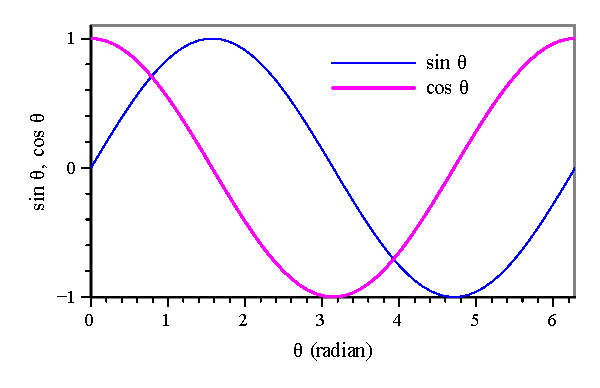
\includegraphics[width=0.75\linewidth]{fig3_1}
\caption[ % Short title which ia appear in figures list
توابع سینوس و کسینوس در یک دورهٔ تناوب]{ % عنوان بلند که زیر شکل می‌آید
توابع سینوس 
(\textcolor{blue}{منحنی نازک}) 
و کسینوس 
(\textbf{\textcolor{magenta}{منحتی ضخیم}}) 
در یک دورهٔ تناوب برحسب زاویه.}
\label{fig3:1}
\end{figure}

شکل~%
\ref{fig3:1} 
نمونه‌ای ساده است که توابع سینوس و کسینوس را در یک دورهٔ تناوب نشان می‌دهد. راهنمای شکل حتی در چاپ سیاه سفید قابل استفاده است. محورها به گونه‌ای مدرج شده اند که پیدا کردن مقادیر ساده است و در عین حال شلوغ نیستند.

وقتی جزییات یک شکل زیاد نباشد، می‌توان عرض آن را کاهش داد و عنوان را کنار آن آورد. شکل~%
\ref{fig3:2} 
همان شکل~%
\ref{fig3:1} 
است که عرض آن کاهش یافته است. اما اندازه قلم به همان نسبت بزرگ شده تا اعداد و نوشته‌ها واضح باشند.

\begin{figure}[!tbhp] % Fig. 3:2
\thisfloatsetup{capbesideposition={center,outside},capbesidewidth=6cm,facing=yes}
\fcapside[\FBwidth]{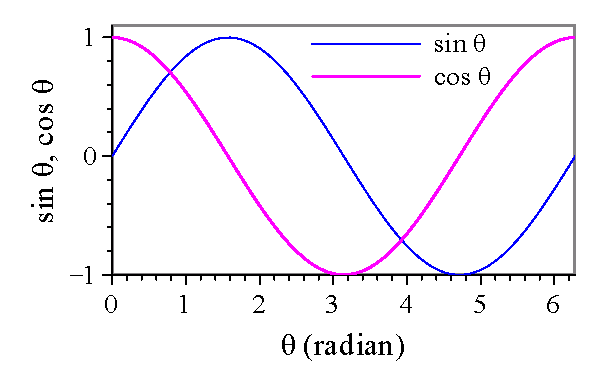
\includegraphics[width=\linewidth]{fig3_2}}{
\caption[ % Short title which ia appear in figures list
توابع سینوس و کسینوس در یک دورهٔ تناوب]{ % عنوان بلند که زیر شکل می‌آید
توابع سینوس 
(\textcolor{blue}{منحنی نازک}) 
و کسینوس 
(\textbf{\textcolor{magenta}{منحتی ضخیم}}) 
در یک دورهٔ تناوب برحسب زاویه. عرض شکل کاهش یافته تا عنوان کنار شکل جا شود.}
\label{fig3:2}}
\end{figure}

همیشه در انتخاب نسبت ابعاد شکل آزاد نیستیم. مثلاً در تصاویر میکروسکپی که با سی‌سی‌دی ثبت می‌شوند، این نسبت براساس سخت‌افزار مشخص می‌شود و نباید آن را تغییر داد. شکل~%
\ref{fig3:3} 
نمونه‌ای از این تصاویر است. شما فقط می‌توانید اندازه شکل را به گونه‌ای تنظیم کنید که همه چیز واضح باشد. فراموش نکنید که این تصاویر باید با میله مقیاسی مدرج شوند که مقیاس واقعی آنها را مشخص کند.

\begin{figure}[!tbhp] % Fig. 3:3
\centering
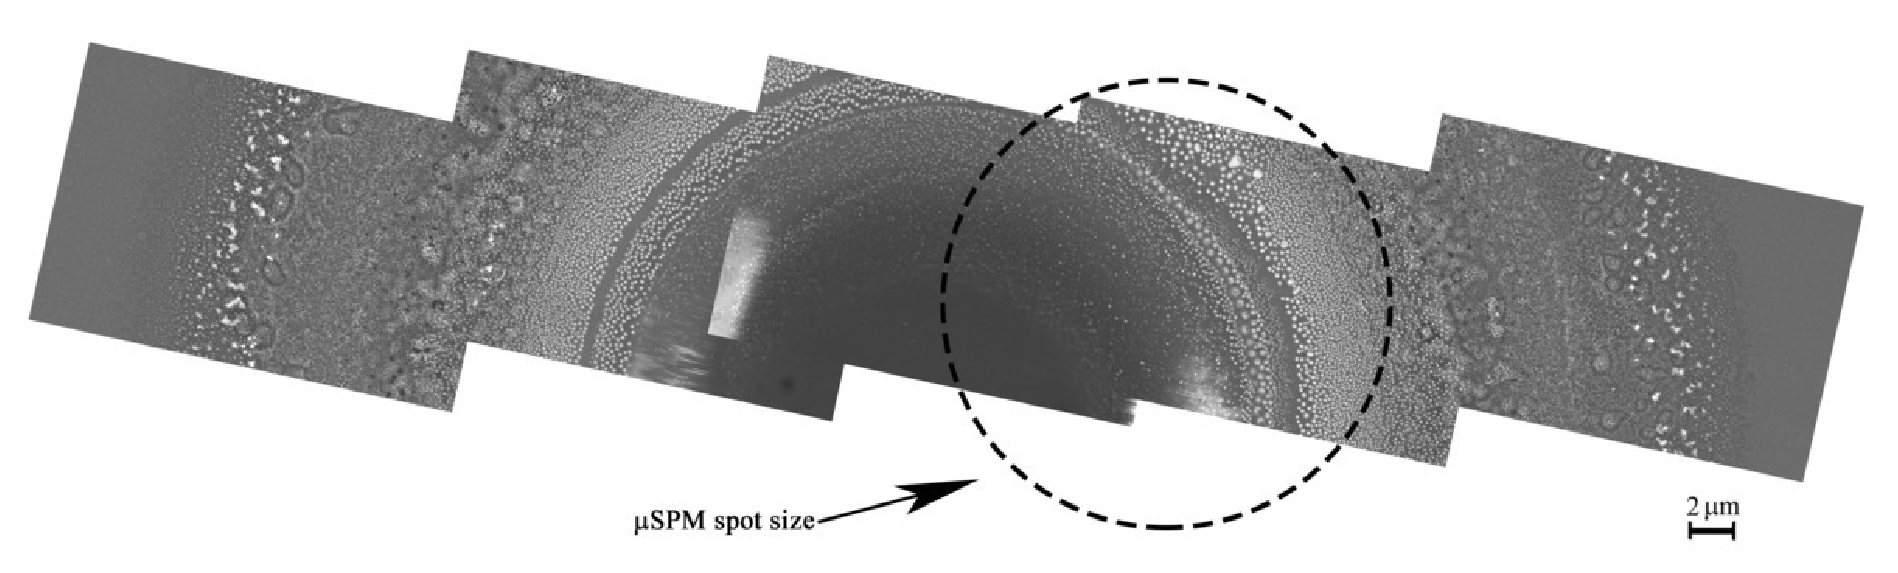
\includegraphics[width=0.9\linewidth]{fig3_3}
\caption[ % Short title which ia appear in figures list
تصویر میکروسکوپی الکترونی از نانوذرات نقره در شیشه تبادل‌یون شده]{ % عنوان بلند که زیر شکل می‌آید
تصویر میکروسکوپی الکترونی از نانوذرات نقره در سطح و ماتریس شیشه تبادل‌یون شدهٔ سودا\dash لایم، برگرفته از مرجع 
\citenum{Ahangary2010}. 
این تصویر عریض از کنارهم قرار دادن و منطبق کردن تعدادی تصویر ساخته شده است.}
\label{fig3:3}
\end{figure}

گاهی نیاز است بیش از یک نمودار یا تصویر در یک شکل گنجانده شوند. شکل~%
\ref{fig3:4} 
چنین نمونه‌ای را نشان می‌دهد. اگر بتوان نسبت ابعاد را به دلخواه انتخاب کرد، بهتر است برای دو شکل قدی کنار هم، نسبت ارتفاع به طول
$1.4$ 
باشد. این نسبت برای سه شکل قدی کنار هم، 
$1.7$ 
است. به این ترتیب نسبت ابعاد هر شکل و کل مجموعه تا حد ممکن مقداری نزدیک به نسبت طلایی خواهند داشت.

\begin{figure}[!tbhp] % Fig 3:4
	\begin{subfigure}[b]{0.35\linewidth}
	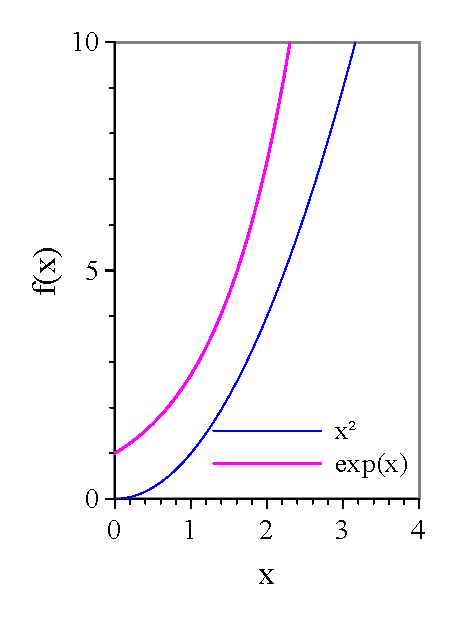
\includegraphics[width=\linewidth]{fig3_4a.eps}
	\caption{}
	\end{subfigure}\qquad
	\begin{subfigure}[b]{0.35\linewidth}
	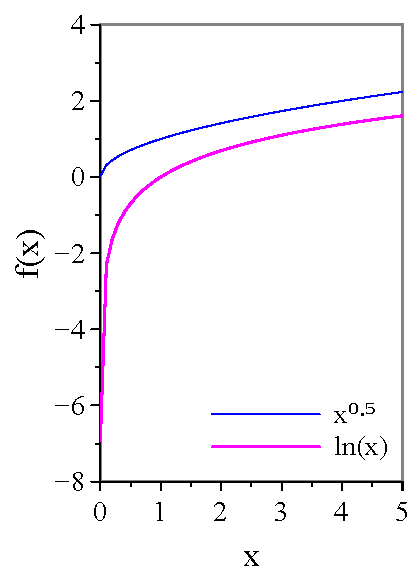
\includegraphics[width=\linewidth]{fig3_4b.eps}
	\caption{}
	\end{subfigure}
\caption[ % Short title which ia appear in figures list
مقایسه رشد سریع تابع نمایی با مربع و رشد کند لگاریتم با جذر]{ % عنوان بلند که زیر شکل می‌آید
(آ) مقایسه رشد سریع تابع نمایی 
(\textbf{\textcolor{magenta}{منحتی ضخیم}}) 
نسبت به توان دوم (مربع) 
(\textcolor{blue}{منحنی نازک}).
(ب) مقایسه رشد کند تابع لگاریتم 
(\textbf{\textcolor{magenta}{منحتی ضخیم}}) 
در مقایسه با جذر 
(\textcolor{blue}{منحنی نازک}).}
\label{fig3:4}
\end{figure}

همیشه نسبت ابعاد در اختیار ما نیست. حتی ممکن است بخواهیم دو شکل با نسبت ابعاد نامساوی را کنار هم بیاوریم. در این موارد بهتر است ارتفاع شکل‌ها را تنظیم کنیم و اجازه دهیم با طول نامساوی کنار هم قرار گیرند، شکل~%
\ref{fig3:5}.


\begin{figure}[!tbhp] % Fig 3:5
	\begin{subfigure}[b]{0.25\linewidth}
	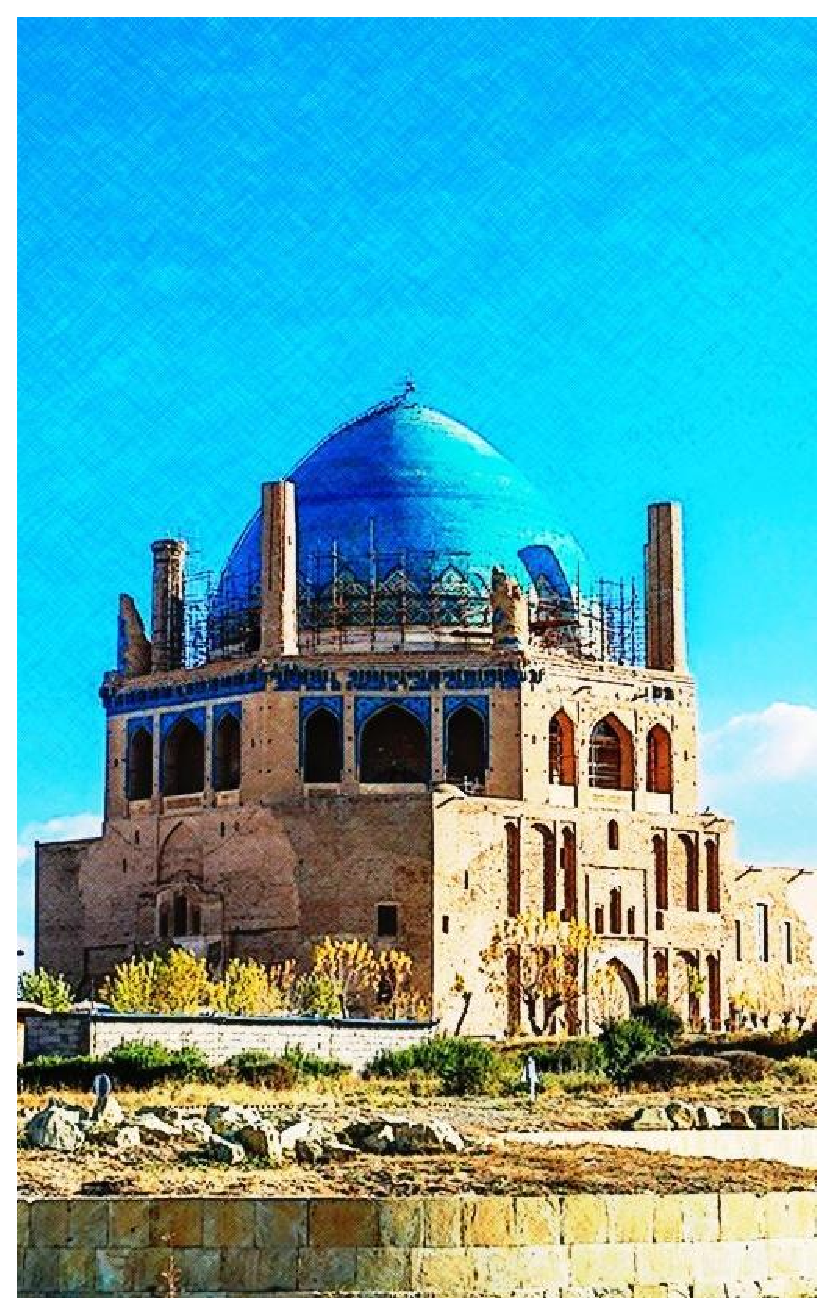
\includegraphics[height=6cm]{fig3_5a.eps}
	\caption{}
	\end{subfigure}\qquad
	\begin{subfigure}[b]{0.55\linewidth}
	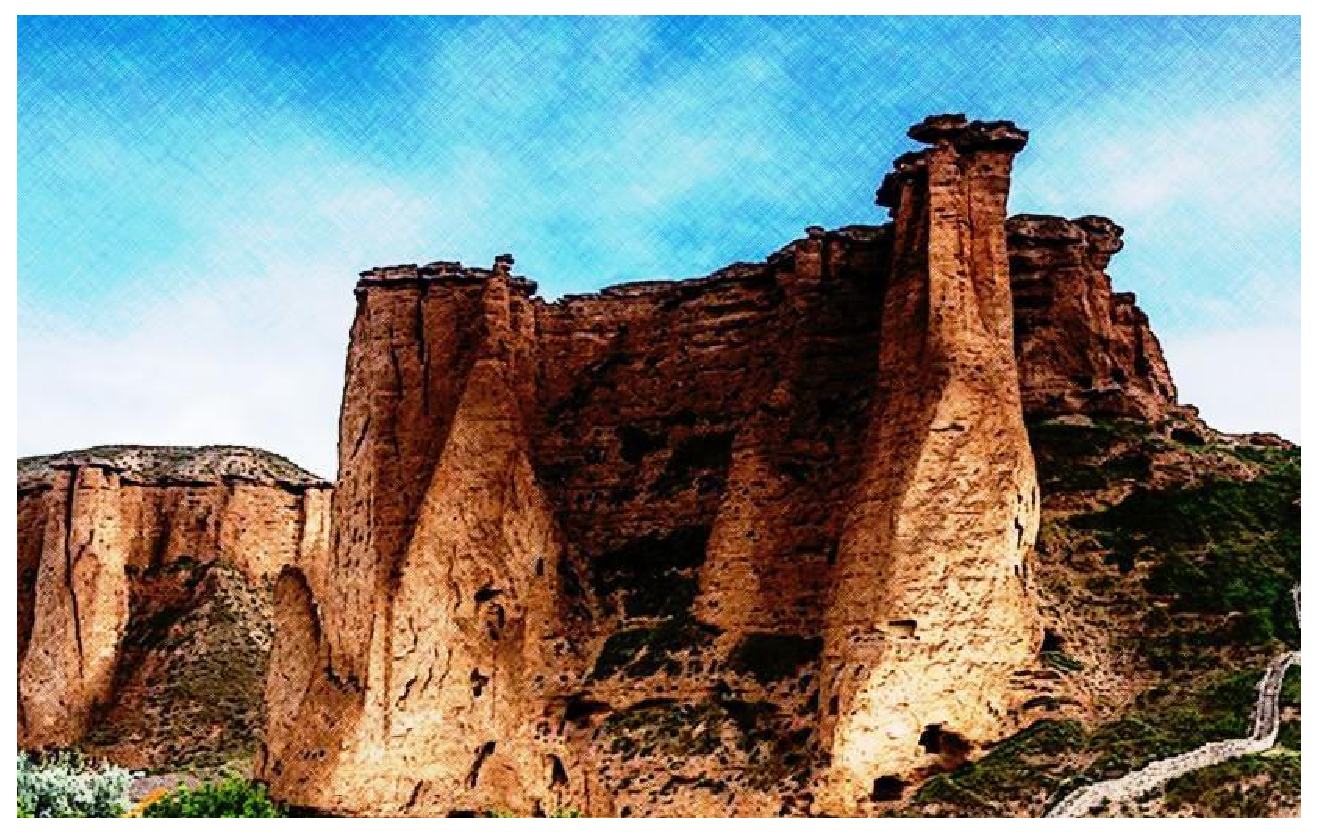
\includegraphics[height=6cm]{fig3_5b.eps}
	\caption{}
	\end{subfigure}
\caption[ % Short title which ia appear in figures list
تصاویری از جاذبه‌های گردشگری زنجان]{ % عنوان بلند که زیر شکل می‌آید
تصاویری از جاذبه‌های گردشگری استان زنجان، (آ) گنبد آجری سلطانیه، (ب) دودکش جن در نزدیکی شهرستان ماهنشان.}
\label{fig3:5}
\end{figure}

گاهی با شرایطی روبرو هستیم که سه نمودار مربوط به هم داریم که می‌خواهیم آنها را در قالب یک شکل ترکیب کنیم. جزئیات شکل‌ها آنقدر زیاد است که نمی‌توان آنها را کوچک کرد و هر سه را در یک سطر کنار هم چید. ترجیح می‌دهیم آنها را در یک ساختار 
$2\times2$ 
جای دهیم. اما سه شکل بیشتر نداریم و جای خالی چهارم زیبا نخواهد بود. در این موارد می‌توان جای خالی را با عنوان شکل‌ها پر کرد. شکل~%
\ref{fig3:6} 
نمونه‌ای از این شرایط را نشان می‌دهد.

\begin{figure}[!tbhp] % Fig 3:6
  \begin{subfloatrow}[2]
    \floatrowsep\quad
    \ffigbox{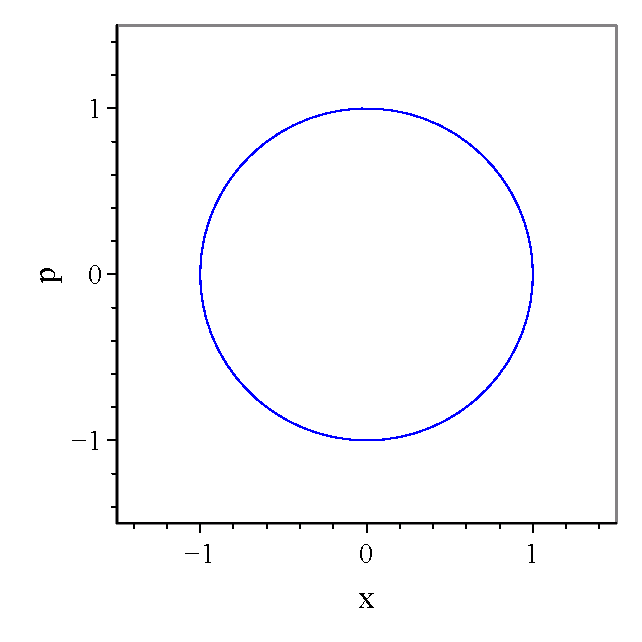
\includegraphics[width=0.45\textwidth]{fig3_6a.eps}}{\subcaption{}}
    \ffigbox{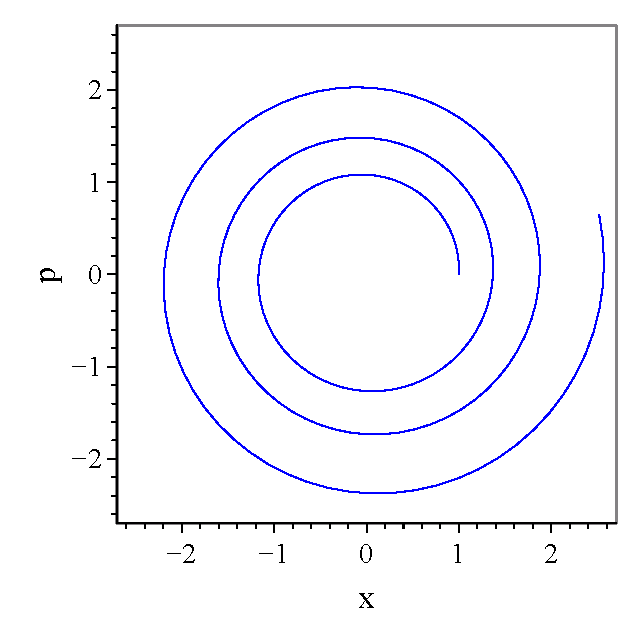
\includegraphics[width=0.45\textwidth]{fig3_6b.eps}}{\subcaption{}}
  \end{subfloatrow}
  \begin{subfloatrow*}[2]
    \floatrowsep\quad
    \ffigbox{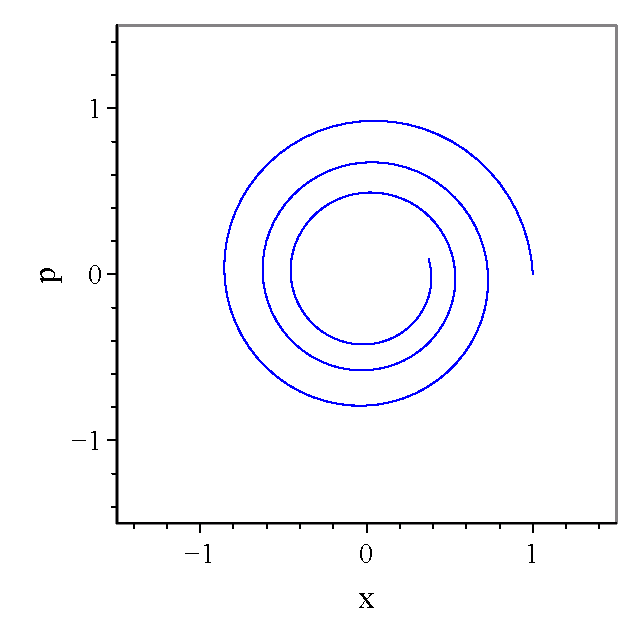
\includegraphics[width=0.45\textwidth]{fig3_6c.eps}}{\subcaption{}}
    \captionsetup{position=top}
    \ffigbox[][][t]{}{
    \RawCaption{\caption[ % Short title which ia appear in figures list
منحنی فاز نوسانگر در سه حالت ایده‌آل، واداشته بدون اتلاف، و اتلافی]{ % عنوان بلند که زیر شکل می‌آید
(آ) منحنی فاز نوسانگر در شرایط ایده‌آل و بدون اتلاف که انرژی ثابت است و نمودار فاز در واحدهای کاهیده دایره‌ای با شعاع واحد است، (ب) منحنی فاز نوسانگر واداشته با اتلاف ناچیز که انرژی آن با زمان افزایش می‌یابد به‌صورت مسیری مارپیچ است که شعاع آن رو به افزایش است. (ج) منحنی فاز نوسانگر اتلافی که انرژی با زمان کاهش می‌یابد و شعاع مسیر مارپیچ به مرور کاهش می‌یابد.}
    \label{fig3:6}}}
  \end{subfloatrow*}
\end{figure}

پیش می‌آید که تعداد زیادی نمودار مرتبط به هم داریم و مایلیم آن‌ها را کنار هم نشان دهیم، مثلاً شکل~\ref{fig3:7}. این نمودارها ممکن است جنبه‌های مختلف یک حل یا شبیه‌سازی را نشان دهند که مایل باشیم همزمان دیده شوند. اما رسم آنها کنار هم سبب شود خیلی کوچک نمایش داده شوند و جزئیات قابل مشاهده نباشد. یک راه‌حل ابتکاری این است که نمودارها را طوری کنار هم بچینیم که محورهای افقی و عمودی مشابه را بتوان به‌صورت مشترک رسم کرد. به این ترتیب با حذف محورهای تکراری بخشی از فضا آزاد می‌شود و می‌توانید نمودارها را اندکی بزرگ‌تر و واضح‌تر رسم کنید. در این مورد بهتر است نمودارها را همسان و همانند هم رسم کنید و کار برش بخش‌های اضافی محورها را در خود 
\latex 
انجام دهید تا هماهنگ کردن تصاویر ساده‌تر شود.

\begin{figure}[!tbhp] % Fig 3:7 
  \begin{subfloatrow}[3]
    \ffigbox{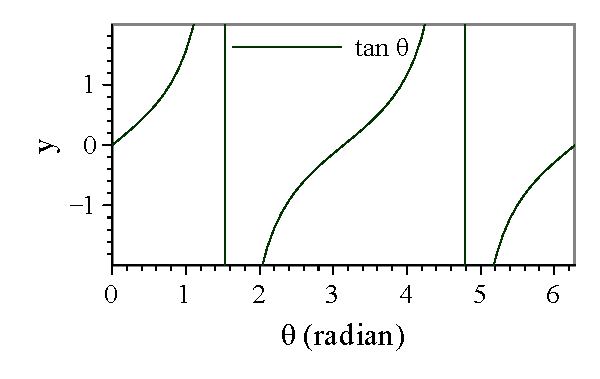
\includegraphics[width=1.26\linewidth,trim= 0 1.5cm 0 0,clip]{fig3_7a.eps}}{}~~~~~~~~~
    \ffigbox{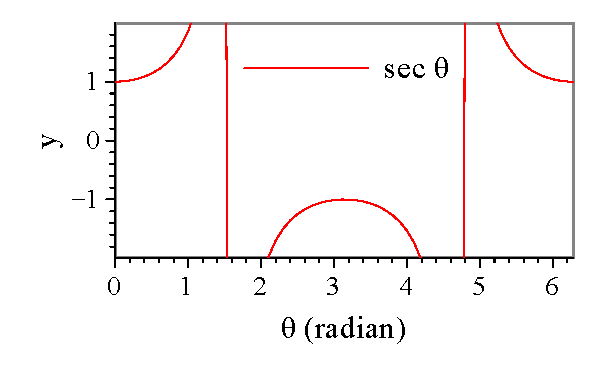
\includegraphics[width=1.06\linewidth,trim= 1.5cm 1.5cm 0 0,clip]{fig3_7b.eps}}{}
    \ffigbox{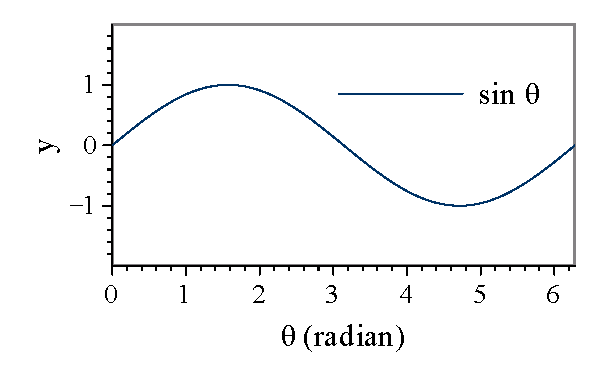
\includegraphics[width=1.06\linewidth,trim= 1.5cm 1.5cm 0 0,clip]{fig3_7c.eps}}{}
  \end{subfloatrow}
  \begin{subfloatrow}[3]
    \ffigbox{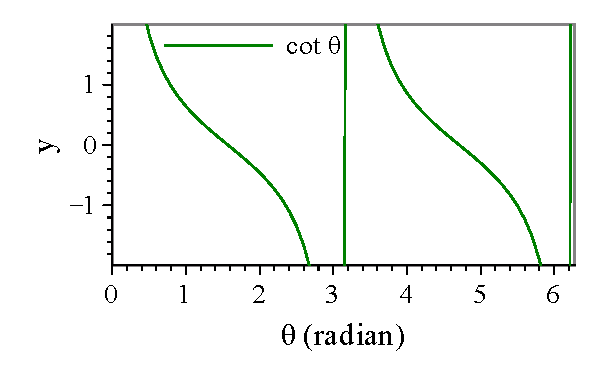
\includegraphics[width=1.26\linewidth,trim= 0 0 0 0,clip]{fig3_7d.eps}}{}~~~~~~~~~
    \ffigbox{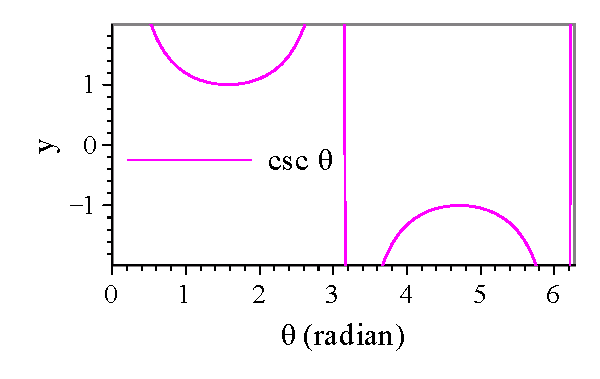
\includegraphics[width=1.06\linewidth,trim= 1.5cm 0 0 0,clip]{fig3_7e.eps}}{}
    \ffigbox{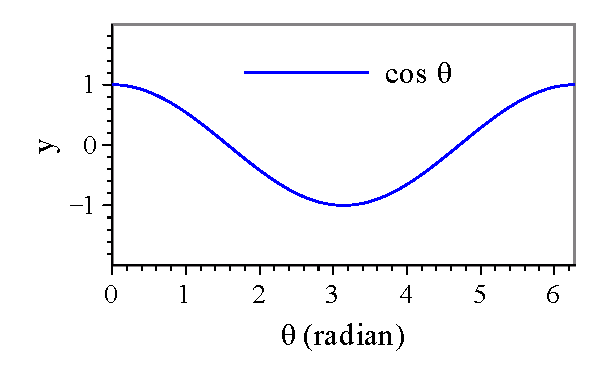
\includegraphics[width=1.06\linewidth,trim= 1.5cm 0 0 0,clip]{fig3_7f.eps}}{}
  \end{subfloatrow}
  \RawCaption{\caption[ % Short title which ia appear in figures list
منحنی تغییرات توابع مثلثاتی در یک دوره تناوب]{ % عنوان بلند که زیر شکل می‌آید
منحنی تغییرات تابع (بالا راست) سینوس، (بالا وسط) سکانت، (بالا چپ) تانژانت، (پایین راست) کسینوس، (پایین وسط) کسکانت، و (پایین چپ) کتانژانت در یک دورهٔ تناوب.}
  \label{fig3:7}}
\end{figure}

وضعیت‌هایی پیش می‌آید که می‌خواهید یک نقشه یا طرح مهم با جزئیات فراوان را نشان دهید و نمایش آن حتی به صورت تنها (نظیر شکل~%
\ref{fig3:1}) 
به اندازه کافی بزرگ و واضح نیست. این شرایط وقتی پیش می‌آید که نسبت طول به ارتفاع شکل بزرگتر است. در این موارد می‌توانید شکل را $90^\circ$ بچرخانید و آن را تنها در یک صفحه کامل بیاورید، شکل~%
\ref{fig3:8}. 
به این ترتیب طول شکل در امتداد ارتفاع صفحه کاغذ که بزرگ‌تر است قرار می‌گیرد و شکل بزرگ‌تر و واضح‌تر دیده می‌شود.

\begin{sidewaysfigure} % Fig. 3:8
\centering

\includegraphics[width=\linewidth]{fig3_8}
\caption[ % Short title which ia appear in figures list
نقشه راهنمای شهر زنجان]{ % عنوان بلند که زیر شکل می‌آید
نقشه راهنمای شهر زنجان، اداره میراث فرهنگی، صنایع دستی و گردشگری استان زنجان.}
\label{fig3:8}
\end{sidewaysfigure}

در این الگو برای کنار هم چیدن شکل‌ها و جدول‌ها، همزمان از بسته‌های 
\lr{subfigure} و \lr{floatrow} \latex 
استفاده شده است. می‌توانید ترکیبات پیچیده‌تر را با مطالعهٔ راهنمای این دو بسته‌ ایجاد کنید. روش ساده‌تر این است که از هوش مصنوعی کمک بگیرید و به دلخواه خودتان ترکیبات پیچیده‌تری را ایجاد کنید. این الگو تسلیم خلاقیت و ابتکار شما است و قصدی برای محدود کردن شما ندارد.


\section{اضافه کردن جدول‌ها}
ممکن است 
\thesis 
شما اصلاً شامل شکل و جدول نباشد. در این صورت به فهرست اشکال و جداول نیز نیاز ندارد. این الگو به‌صورت خودکار با اضافه شدن اولین شکل و جدول، به ترتیب فهرست اشکال و جدوال را به 
\thesis 
اضافه می‌کند. 

جدول~%
\ref{tab3:1} 
نمونه‌ای از یک جدول است که با حذف خطوط افقی و عمودی به زیبایی آن افزوده شده است.

\begin{table}[!htbp] % Table 3:1
\caption{\small
برخی پیشوندها در دستگاه اندازه‌گیری 
\lr{SI}.}\label{tab3:1}
\begin{center}\small\begin{tabular}{rcl} 
\hline\noalign{\smallskip}
\textbf{
نام پیشوند} & \textbf{حرف اختصاری} & \textbf{مقدار}\\[4pt] 
\hline\noalign{\smallskip}
دسی
& $\mathrm{d}$ & $10^{-1}$\\
سانتی
& $\mathrm{c}$ & $10^{-2}$\\
میلی
& $\mathrm{m}$ & $10^{-3}$\\
میکرو
& $\mu$        & $10^{-6}$\\[4pt]
\hhline{===}
\end{tabular}\end{center}
\end{table}

برخی مواقع لازم است که دو یا چند خانه جدول باهم ادغام شوند. مثلاً در جدول~%
\ref{tab3:2}، 
دو خانه اول در سطر اول سرایند جدول ادغام شده‌اند. در دو ستون بعدی نیز خانه‌ها در دو سطر متوالی با هم ادغام شده اند تا سرآیند جدول زیباتر شود.

\begin{table}[!htbp] % Table 3:2
\small\caption{
برخی مقادیر و ثابت‌های فیزیکی.}
\label{tab3:2}
\begin{tabular}{rcll} 
\hline\noalign{\smallskip}
\multicolumn{2}{c}{\textbf{
ثابت‌های فیزیکی}} & 
\multirow{2}{*}{\textbf{مقدار}} & 
\multirow{2}{*}{\textbf{نماد}}\\[4pt]
\hhline{--} \noalign{\smallskip}
نام & توضیحات \\[4pt]
\hline \noalign{\smallskip}
سرعت نور & در خلا &
$3 \times 10^8\unit{m/s}$ & $c$\\
\multicolumn{2}{r}{
ثابت پلانک} & 
$6.626 \times 10^{-34}\unit{Js}$ & $h$\\
جرم الکترون & در حالت سکون & 
$9.109 \times 10^{-31}\unit{kg}$ & $m_\mathrm{e}$\\[4pt]
\hline
\end{tabular}
\end{table}

همانند شکل‌ها، ممکن است با جدول‌هایی روبرو شوید که تعداد زیادی ستون داشته باشند. به‌عبارتی تعداد ستون‌ها و عرض آنها در مجموع بیش از عرض صفحه باشد. بهتر است برای جادادن چنین جداولی در صفحه، جدول را $90^\circ$ بچرخانید و یک صفحه کامل به آن اختصاص دهید. کافیست به‌جای محیط 
\lr{table} 
از محیط 
\lr{sidewaystable} 
استفاده کنید،~\ref{tab3:3}.

\begin{sidewaystable} % Table 3:3
\small\caption[ % Short title which ia appear in figures list
حالت‌های متنوع کلاس\dash سند \lr{`iasbs-thesis'}.]{ % عنوان بلند که زیر شکل می‌آید
حالت‌های متنوع کلاس\dash سند \lr{`iasbs-thesis'} و چیدمان صفحات برمبنای انتخاب آنها.}
\label{tab3:3}
\newcommand{\vr}[1]{\rotatebox{90}{\small #1}}
\begin{tabular}{rc ccccc c ccc cccc c} 
\hline\noalign{\smallskip}
\multirow{2}{*}{\parbox{6em}{\vspace{8em}\centering\textbf{
نوع سند}}} & 
\multirow{2}{*}{\parbox{10em}{\vspace{8em}\centering\textbf{
گزینه‌های انتخاب شده}}} & 
\multicolumn{14}{c}{\textbf{شمارهٔ صفحه}$\,\!^*$}\\[4pt] 
\hhline{~~----- - --- ---- -}\noalign{\smallskip}
&& \vr{جلد} & \vr{عنوان فارسی} & \vr{عنوان انگلیسی} & \vr{شناسنامه} & \vr{کپی‌رات} & 
   \vr{بسم الله الرحمن الرحیم} & 
   \vr{اعلامیه} & \vr{تأییدیه فارسی} & \vr{تأییدیه انگلیسی} & 
   \vr{تقدیم به} & \vr{قدردانی} & \vr{چکیده فارسی} & \vr{چکیده انگلیسی} & 
   \vr{فهرست‌ها}\\
\hline \noalign{\smallskip}   
پیش‌نویس رسالهٔ دکتری & \lr{phd + review} & 
1 & 3 & 4 & 5 & 6 &   8 &   9 & 10 & 11 &   12 & 13 & 14 & 15 & 16\\[4pt]
رسالهٔ دکتری & \lr{phd} & 
\lr{ix} & 1 & \lr{vii} & 2 & \lr{iii} &   3 &   5 & 7 & \lr{v} &   9 & 11 & 13 & \lr{i} & 15\\[4pt]
پیشنهاد رسالهٔ دکتری & \lr{phd + proposal} &
- & 1 & \lr{} & 2 & \lr{i} &   3 &   - & - & - &   - & - & 5 & - & 7\\[4pt]
پیش‌نویس پایان‌نامهٔ کارشناسی ارشد & \lr{master + review} &
1 & 3 & 4 & 5 & - &   6 &   - & 7 & 8 &   10 & 11 & 12 & 13 & 14\\[4pt]
پایان‌نامهٔ کارشناسی ارشد & \lr{master} & 
\lr{xii} & 1 & \lr{v} & 2 & - &   3 &   - & 5 & \lr{iii} &   7 & 9 & 11 & \lr{i} & 13\\[4pt]
گزارش پروژه کارشناسی & \lr{-} &
- & 1 & \lr{i} & - & - &   - &   - & - & - &   - & - & 3 & \lr{} & 5\\[4pt]
\hline \noalign{\smallskip}
\multicolumn{14}{r}{$\,\!^*$
شمارهٔ یونانی مشخص می‌کند آن صفحه در انتهای \thesis می‌آید.}
\end{tabular}
\end{sidewaystable}


\section{تسهیل نگارش اصطلاحات علمی}
در یک متن علمی، واژگان و اصطلاحات زیادی وجود دارد که باید به نحو مناسب از معادل فارسی یا  مخفف آنها استفاده کنید. گاهاً معادل فارسی این اصطلاحات خیلی طولانی است و برای آنها همانند انگلیسی مخفف نداریم یا شما مطمئن نیستید که مخففی که قصد استفاده از آن را دارید با اقبال داوران روبرو شود. در اینجا چند مثال از دستورات 
\latex 
می‌آوریم که می‌توانید ابتدای فایل اصلی 
\thesis (\lr{``main.tex"}) 
قبل از محیط 
$\backslash\texttt{begin\{documnet\}}$
بیاورید و برای تسهیل نگارش چنین اصلاحاتی از آنها استفاده کنید. 

برای مثال در انگلیسی معمولاً 'روش افت‌وخیز روندزدایی شده%
\LTRfootnote{Detrended Fluctuation Analysis (DFA)}` 
به اختصار 
\lr{DFA} 
نوشته می‌شود. تکرار کردن این اصطلاح طولانی و درست نوشتن فاصله‌ها و نیم‌فاصله‌های آن دشوار و خسته کننده است. اگر دستور کوتاهی در 
\latex 
این اصطلاح طولانی را برای ما تولید کند خیلی راحت‌تر است. کافی است کد زیر در ابتدای کد اصلی اضافه شود تا دستور 
'$\backslash\texttt{dfa}$` 
این کار را برایمان انجام دهد،
\begin{latin}
\noindent$\backslash\texttt{newcommand}\{\backslash\texttt{dfa}\}\{
\mbox{\small\rl{
افت‌وخیز روندزدایی شده}}%
\!\backslash\texttt{xspace}\}$
\end{latin}

مثال دیگری که می‌توان زد اصطلاح 'دینامیک مولکولی%
\LTRfootnote{Molecular Dynamics (MD)}` 
است. در انگلیسی این اصطلاح را به اختصار 
\lr{MD} 
می‌نویسند. ممکن است در زمان نگارش 
\thesis 
واژهٔ 'دینامول` به عنوان مخفف فارسی 'دینامیک مولکولی` به ذهنمان برسد، اما از نظر مساعد داوران مطمئن نباشیم. راه‌حل تعریف دستور 
'$\backslash\texttt{md}$`
در ابتدای فایل اصلی است،
\begin{latin}
\noindent$\backslash\texttt{newcommand}\{\backslash\texttt{md}\}\{
\mbox{\small\rl{
دینامول}}%
\!\backslash\texttt{xspace}\}$
\end{latin}
\noindent
به این ترتیب هم نگارش آن به اندازه نسخهٔ انگلیسی ساده است و هم فرصت خواهیم داشت در آینده در نحوه نگارش آن تجدید نظر کنیم.

مورد آخر وقتی است که می‌خواهیم یک واژه را به صورت خاصی بنویسیم. مثلاً برای خوانش درست اعراب‌گذاری کنیم، یا جلوه هنری یا فانتزی به آن بدهیم و این کار پیچیدگی‌هایی دارد که نمی‌خواهیم هر بار آن را تکرار کنیم. نمونه‌های آن لوگوهای
\latex، \xelatex، 
و 
\xepersian 
به فارسی است که از نمونه انگلیسی آنها برداشت شده است (
\LaTeX، \XeLaTeX، و \XePersian). 
این مثال اگرچه جایی در متن 
\thesis{ٔ} 
شما ندارد، اما قابلیت‌هایی را در نگارش متن نمایش می‌دهد که ممکن است به کارتان بیاید. برای مشاهده تعریف دستوراتی که این لوگوهای فارسی را تولید می‌کند، به فایل 
'$\texttt{main.tex}$` 
مراجعه کنید.


\section{یاداشت‌گذاری}
زیاد پیش می‌آید که توصیه‌هایی از استاد راهنما یا مشاور دریافت کنید یا نکاتی به ذهنتان برسد، اما همان موقع نتوانید آنها را رفع کنید و مایل باشید برای یادآوری کارهایی که باید انجام دهید، در متن یادداشت بگذارید. این کار با بسته \lr{easyReview} قابل انجام است. مزیت این بسته آن است که در نوار ابزار نرم‌افزار استودیوی‌تک%
\LTRfootnote{TeXstudio} 
از پیش گزینه‌هایی برای فراخوانی دستورات این بسته وجود دارد. با این بسته می‌توانید کارهای زیر را انجام دهید:

\begin{itemize}
\item 
پیام 
\alert{%
هشداری} را در متن نمایش دهید تا فراموش نشود.
\item 
\add{%
متن جدید اضافه شده به متن اصلی} را مشخص کنید.
\item 
متن حذف شده از متن اصلی
\remove{%
متن اضافی} را مشخص کنید. 
\item
مشخص کنید که کجا 
\replace{%
متنی جایگزین}{متنی دیگر} شده است.
\item
قسمتی از
\highlight{%
متن را هایلایت} کنید تا بعداً به آن توجه کنید.
\item 
توضیحاتی را به متن اصلی اضافه کنید: 
\comment{%
مثلاً این جمله نیاز به کامنت و توضیح دارد که در جعبه زیر متن ظاهر می‌شود.}{نکته: هر زمان مایل باشید می‌توانید توضیحات و تاریخچه تصحیحات را با درج دستور 
\latex $\backslash\texttt{setreviewsoff}$
موقتا از نتیجه نهایی حذف کنید تا بتوانید ظاهر نسخه نهایی را بعد از اعمال تصحیحات ببینید.}

این الگو فقط در حالت مرور 
(\lr{review}) 
در فایل کلاس تز دانشگاه
(\lr{iasbs-thesis.cls}) 
تصحیحات را نشان می‌دهد و در حالت عادی آنها را تا حد امکان حذف می‌کند تا به اشتباه در متن نهایی 
\thesis 
باقی نمانند.
\end{itemize}


\section{الگوریتم}
الزامی ندارد در این فصل الگوریتم کارتان را قدم به قدم توضیح دهید. به‌خصوص اگر از الگوریتم شناخته شده‌ای استفاده می‌کنید، توضیحات کلی همراه با مرجع مناسب کفایت می‌کند. اما اگر مُبدع الگوریتم هستید، بهتر است آن را قدم به قدم شرح دهید. برای تسهیل کار خواننده می‌توانید، همراه با توضیحات از الگوریتم یا روندنما (فلوچارت) استفاده کنید. نحوه نوشتن یک الگوریتم به صورت راست‌چین مشابه الگوریتم~%
\ref{alg3:rtl} 
است. در اینجا کلیدواژه‌های متداول، مثل 
\lr{`\textbf{for}'} 
با معادل فارسی آنها جایگزین شده اند تا خوانایی الگوریتم افزایش یابد.
\begin{algorithm}[H] % Algorithm 1 - 'H' forces latex to put algorithm here!
\caption{\small
محاسبهٔ تابع فاکتوریل.}
\label{alg3:rtl}
\begin{algorithmic}[1] \small % وجود کروشه سبب شماره‌گذاری خطوط الگوریتم می‌شود
\State 
مقدار پارامتر $N$ مشخص شود.
\If{$N<0$}
  \State 
محاسبهٔ تابع فاکتوریل ممکن نیست!
\Else
  \State 
مقدار اولیه $f=1$ مشخص شود.
  \For{$n$ 
از $1$‌ تا $N$}
    \State $f \gets nf$ \Comment{$f$ 
را $n$ برابر می‌کند.}
  \EndFor
  \State 
نتیجهٔ فاکتوریل برابر مقدار $f$ است.
\EndIf
\end{algorithmic}
\end{algorithm}

در عین حال می‌توان تمام الگوریتم را چپ‌چین و بیشتر به زبان ریاضی نوشت و از کلمات کلیدی شناخته شده در شبه کدها استفاده کرد. در الگوریتم 
\ref{alg3:ltr} 
سعی شده است کلمات کلیدی پُر استفاده گنجانده شوند.

ترسیم روندنما نسبت به نگارش الگوریتم زحمت بیشتری دارد. برای ترسیم روندنما از نرم‌افزارهای ترسیم برداری%
\LTRfootnote{vector graphics software}
نظیر 
\lr{INKSCAPE} و \lr{IPE} 
یا محیط‌های آنلاین مختص رسم فلوچارت استفاده کنید. در محیط \latex نیز می‌توانید از بستهٔ 
\lr{tikz} 
به این قصد استفاده کنید.

\begin{algorithm}[H] % Algorithm 2
\caption{\small
نمونه‌ای از الگوریتم به صورت چپ‌چین}
\label{alg3:ltr}
\begin{latin}\small
\begin{algorithmic}[1] % وجود کروشه سبب شماره‌گذاری خطوط الگوریتم می‌شود
\Require $x \in \{0,1\}$
\Ensure $y \in \{1,2\}$
\State\rl{
یک خط از کد الگوریتم مثلاً تنظیم مقادیر اولیه}
\Statex\rl{
دنبالهٔ خط قبلی بدون شماره‌گذاری}
\State\Call{Proc}{a1, a2} \Comment{\rl{
فراخوانی یک تابع.}}
\While{condition}
  \State\rl{بدنهٔ حلقه}
\EndWhile
%
\For{$n = 1, \dots, 10$}
  \State\rl{بدنهٔ حلقه}
\EndFor
%
\Repeat
  \State\rl{بدنهٔ حلقه}
\Until{$n > 10$}
%
\If{condition}
  \State\rl{بدنهٔ شرط}
\ElsIf{condition}
  \State\rl{بدنهٔ شرط}
\Else
  \State\rl{بدنهٔ شرط}
\EndIf
  \State $x \gets x + 1$ \Comment{\rl{
افزایش یک واحدی $x$.}}
\State $y \gets y + 1$ \Comment{\rl{
افزایش یک واحدی $y$.}}
\State\Return $y$ \Comment{\rl{
بازگرداندن نتیجهٔ اجرای الگوریتم.}}
\end{algorithmic}
\end{latin}
\end{algorithm}


